% tMAMguide.tex
% v3.3 released August 2008

\documentclass[]{tMAM2e}
\renewcommand{\baselinestretch}{1.175}
\begin{document}

\doi{10.1080/1745973YYxxxxxxxx}
 \issn{1745-9745} \issnp{1745-9737}

  \jnum{00} \jyear{2008} \jmonth{January}

\markboth{Taylor \& Francis and I.T. Consultant}{Journal of Mathematics and Music}

\articletype{GUIDE}

\title{{\itshape Journal of Mathematics and Music: Mathematical and Computational Approaches to Music Theory, Analysis, Composition and Performance}---\LaTeXe\ style guide for authors (Style 2 + References Style Q)}

\author{Taylor \& Francis$^{\rm a}$$^{\ast}$\thanks{$^\ast$Corresponding author. Email: latex.helpdesk@tandf.co.uk
\vspace{6pt}} and I.T. Consultant$^{\rm b}$\\\vspace{9pt}  $^{\rm a}${\em{4 Park Square, Milton Park, Abingdon,
OX14 4RN, UK}}; $^{\rm b}${\em{Institut f\"{u}r Informatik, Albert-Ludwigs-Universit\"{a}t, D-79110 Freiburg,
Germany}}\\\vspace{9pt}\received{v3.3 released August 2008} }



\maketitle
\bigskip
\begin{abstract}
This guide is for authors who are preparing papers for the Taylor \& Francis journal {\em Journal of Mathematics and Music} ({\it tMAM}\,) using the \LaTeXe\ document preparation system and the Class file {\tt
tMAM2e.cls}, which is available via the journal homepage on the Taylor \& Francis website (see
Section~\ref{FTP}). Authors planning to submit their papers in \LaTeXe\ are advised to use {\tt tMAM2e.cls} as
early as possible in the creation of their files.\bigskip

\begin{keywords}submission instructions; source file coding;
environments; references citation; fonts; numbering {\bf{(Authors: Please provide five to ten keywords taken
from terms used in your manuscript)}}
\end{keywords}
\begin{classcode}F1.1; F4.3 {\bf{(... for example; authors are encouraged to provide some MCS/CCS/AMS Classification codes or CR Category numbers)}}\end{classcode}\bigskip

\newpage

\centerline{\bfseries Index to information contained in this
guide}\bigskip
\hbox to \textwidth{\hsize\textwidth\vbox{\hsize24pc
\hspace*{-12pt} {1.}    Introduction\\
\hspace*{7pt} {1.1.}  The {\it tMAM} document style\\
\hspace*{7pt} {1.2.}  Submission of \LaTeXe articles\\
\hspace*{28pt}        to the journal\\
{2.}    Using {\it tMAM} style\\
\hspace*{10pt}{2.1.}  Landscape pages\\
{3.}    Additional features\\
\hspace*{10pt}{3.1.}  Footnotes to article titles\\
\hspace*{28pt}        and authors' names\\
\hspace*{10pt}{3.2.}  Abstracts\\
\hspace*{10pt}{3.3.}  Lists\\
{4.}    Some guidelines for using\\
\hspace*{10pt}        standard features\\
\hspace*{10pt}{4.1.}   Sections\\
\hspace*{10pt}{4.2.}   Illustrations (figures)\\
\hspace*{10pt}{4.3.}   Tables\\
\hspace*{10pt}{4.4.}   Running headlines\\
\hspace*{10pt}{4.5.}   Maths environments\\
\noindent \hspace*{7pt} {4.6.}   Typesetting mathematics\\
\hspace*{24pt} {4.6.1.}   Displayed mathematics\\
\hspace*{24pt} {4.6.2.}  Bold math italic symbols\\
\hspace*{24pt} {4.6.3.}   Bold Greek\\
\hspace*{24pt} {4.6.4.}   Upright Greek characters  \\
\hspace*{7pt} {4.7.}   Acknowledgements \\} \hspace{-84pt}\vbox{\noindent\hsize24pc
\hspace*{7pt} {4.8.}   Notes \\
\hspace*{7pt} {4.9.}   Appendices \\
\hspace*{7pt} {4.10.}   References \\
\hspace*{34pt} {4.10.1.}   References cited in the\\ \hspace*{74pt}text  \\
\hspace*{34pt} {4.10.2.}   The list of references\\
\hspace*{7pt} {4.11.}   {\it tMAM} macros\\
{5.}    Example of a section heading with\\*
\hspace*{10pt}  {\fontencoding{T1}\scshape\lowercase{small caps}},
   \lowercase{lowercase}, {\it italic}, and bold\\*
\hspace*{10pt}  Greek such as
   ${\bm\kappa}$ \\
{6.}   {\em tMAM} journal style \\
\hspace*{10pt}{6.1.}   Punctuation\\
\hspace*{10pt}{6.2.}   Spelling \\
\hspace*{10pt}{6.3.}   Hyphens, n-rules, m-rules and\\ \hspace*{32pt}minus signs\\
\hspace*{10pt}{6.4.}   References \\
\hspace*{10pt}{6.5.}   Maths fonts\\
\noindent   {7.}   Troubleshooting\\
\hspace*{10pt}{7.1.}   Fixes for coding problems\\
     {8.}   Obtaining the tMAM2e Class file\\
\hspace*{10pt}{8.1}  Via the Taylor \& Francis website\\
\hspace*{10pt}{8.2}   Via e-mail\\\\
      }}
\end{abstract}


\section{Introduction}

Authors are encouraged to submit manuscripts electronically. Electronic submissions for possible publication in  {\itshape Journal of Mathematics and Music} ({\it tMAM}\,) should be sent by e-mail attachment. If e-mail submission is not possible, please send an electronic version on CD or disc, along with three paper copies and one set of high-quality figures for reproduction. {\it tMAM} prefers papers in PDF format created from \LaTeXe\ source files (see Section~1.2).

The layout design for {\it tMAM} has been implemented as a \LaTeXe\ Class file. The {\it tMAM} Class file is
based on {\tt article.cls}. Commands that differ from the standard \LaTeXe\ interface, or which are provided in
addition to the standard interface, are explained in this guide. This guide is not a substitute for the \LaTeXe\
manual itself.

This guide can be used as a template for composing an article for submission by cutting, pasting, inserting and
deleting text as appropriate, using the LaTeX environments provided (e.g. \verb"\begin{equation}",
\verb"\begin{corollary}"). \vspace{6pt}

\noindent{\bf{Please note that the index following the abstract in this guide is provided for information only. An index is not required in submitted papers.}}

\subsection{The {\bi tMAM} document style}

The use of \LaTeXe\ document styles allows a simple change of style (or style option) to transform the appearance
of your document. The tMAM2e Class file preserves the standard \LaTeXe\ interface such that any document that can
be produced using the standard \LaTeXe\ {\tt article} style can also be produced with the {\it tMAM} style.
However, the measure (or width of text) is narrower than the default for {\tt article}, therefore line breaks
will change and long equations may need re-formatting.

When your article appears in the print edition of the {\it tMAM} journal, it is typeset in Monotype Times. As
most authors do not own this font, it is likely that the page make-up will change with the change of font. For
this reason, we ask you to ignore details such as slightly long lines, page stretching, or figures falling out of
synchronization with their citations in the text, because these details will be dealt with at a later stage.


\subsection{Submission of \LaTeXe\ articles to the journal}

Authors are encouraged to submit manuscripts electronically. Electronic submissions should be sent by e-mail attachment. Papers for consideration should be sent to the Editors-in-Chief at the following address: Thomas Noll - Department of Theory and Composition, L'Escola Superior de M\'{u}sica de Catalunya, C/Padilla, 155, Edifici L'Auditori, 08013 Barcelona, Spain (E-mail: tnoll@iua.upf.edu); Robert Peck - School of Music, Louisiana State University, Baton Rouge, LA 70803-2504, USA (E-mail: rpeck@lsu.edu). Authors interested in submitting reviews are encouraged to contact the Reviews Editor in advance. Books to be considered for possible review may also be sent to the Reviews Editor: Julian Hook (Reviews Editor) - Indiana University, Jacobs School of Music, Bloomington, IN 47405, USA (E-mail: juhook@indiana.edu).

A PDF file of manuscripts prepared using \LaTeXe\ should be created from the source files and e-mailed as above together with the source files themselves and any graphics files. If e-mail submission is not possible, please send an electronic version on CD or disc, along with three paper copies and one set of high-quality figures for reproduction.

General Instructions for Authors may be found at

\centerline{\nobreak{\tt{http://www.tandf.co.uk/journals/authors/tmamauth.asp.}}}

Only `open-source' \LaTeXe\ should be used, not proprietary systems such as TCI LaTeX or Scientific WorkPlace. Similarly, Class files such as REVTex4 that produce a document in the style of a different publisher and journal should not be used for preference.

Appropriate gaps should be left for figures, of which original versions and copies should also be supplied.
Authors should ensure that their figures are suitable (in terms of lettering size, etc.) for the reductions they
intend.

Authors who wish to incorporate Encapsulated PostScript artwork directly in their articles can do so by using
Tomas Rokicki's {\tt EPSF} macros (which are supplied with the DVIPS PostScript driver). See Section~\ref{eps},
which also demonstrates how to treat landscape pages. Please remember to supply any additional figure macros you
use with your article in the preamble before \verb"begin{document}". Authors should not attempt to use
implementation-specific \verb"\special"'s directly.

Ensure that any author-defined macros are gathered together in the source file, just before the
\verb"\begin{document}" command.

Please note that, if serious problems are encountered with the coding of a paper (missing author-defined macros,
for example), it may prove necessary to divert the paper to conventional typesetting, i.e. it will be re-keyed.

\section{Using the {\bi tMAM} Class file}

If the file {\tt tMAM2e.cls} is not already in the appropriate system directory for \LaTeXe\ files, either
arrange for it to be put there, or copy it to your working folder. The {\it tMAM} document style is implemented
as a complete document style, {\em not\/} a document style option. In order to use the {\it tMAM} style, replace
{\tt `article'} by {\tt `tMAM2e'} in the \verb"\documentclass" command at the beginning of your document:
%
\begin{verbatim}
\documentclass{article}
\end{verbatim}
%
is replaced by
%
\begin{verbatim}
\documentclass{tMAM2e}
\end{verbatim}
%
In general, the following standard document style options should
{\em not\/} be used with the {\it tMAM} style:
%
\begin{enumerate}
   \item {\tt 10pt}, {\tt 11pt}, {\tt 12pt}---unavailable;
\item oneside (no associated style file)---oneside is the default;
   \item {\tt leqno} and {\tt titlepage}---should not be used;
   \item {\tt singlecolumn}---is not necessary as it is the default style.
\end{enumerate}
%

\subsection{Landscape pages}\label{eps}

If a table or illustration is too wide to fit the standard measure,
it must be turned, with its caption, through 90$^{\circ}$
anticlockwise. Landscape illustrations and/or tables can be produced
directly using the tMAM2e style file using
\verb"\usepackage{rotating}" after \verb"\documentclass{tMAM2e}".
The following commands can be used to produce such pages.
%
\begin{verbatim}
\setcounter{figure}{2}
\begin{sidewaysfigure}
\centerline{\epsfbox{fig1.eps}}
\caption{This is an example of figure caption.}
\label{landfig}
\end{sidewaysfigure}
\end{verbatim}
%
\begin{verbatim}
\setcounter{table}{0}
\begin{sidewaystable}
  \tbl{The Largest Optical Telescopes.}
    \begin{tabular}{@{}llllcll}
    .
    .
    .
  \end{tabular}\label{tab1}
\end{sidewaystable}
\end{verbatim}
%
Before any float environment, use the \verb"\setcounter" command
as above to fix the numbering of the caption. Subsequent captions
will then be automatically renumbered accordingly.


\section{Additional features}

In addition to all the standard \LaTeXe\ design elements, {\it tMAM} style includes a separate command for specifying short versions of the authors' names and the journal title for running headlines on the left-hand (verso) and right-hand (recto) pages, respectively (see Section~\ref{markboth}).  In general, once you have used this additional {\tt tMAM2e.cls} feature in your document, do not process it with a standard \LaTeXe\ style file.

\subsection{Footnotes to article titles and authors' names}

On the title page, the \verb"\thanks" control sequence may be used to produce a footnote to either the title or authors' names.

Footnote symbols should be used in the order: $\dagger$
(coded as \verb"\dagger"),\break $\ddagger$ (\verb"\ddagger"), $\S$ (\verb"\S"),
$\P$ (\verb"\P"), $\|$ (\verb"\|"), $\dagger\dagger$
(\verb"\dagger\dagger"),\break $\ddagger\ddagger$
(\verb"\ddagger\ddagger"),  $\S\S$ (\verb"\S\S"), $\P\P$ (\verb"\P\P"),
$\|\|$ (\verb"\|\|").

Note that footnotes to the text will automatically be assigned the superscript symbols 1, 2, 3,... by the Class file, beginning afresh on each page.\footnote{These symbols will be changed to the style of the journal by the typesetter during preparation of your proofs.}

The title, author(s) and affiliation(s) should be followed by the
 {\verb"\maketitle"} command.

\subsection{Abstracts}

At the beginning of your article, the title should be generated in
the usual way using the {\verb"\maketitle"} command. Immediately
following the title you should include an abstract. The abstract
should be enclosed within an {\tt abstract} environment. For
example, the titles for this guide were produced by the following
source code:
%
\begin{verbatim}

\title{Journal of Mathematics and Music: Mathematical and Computational%
 Approaches to Music Theory, Analysis, Composition and Performance ---%
 \LaTeXe\ style guide for authors \break(Style 2 + References Style Q)}%
\author{Taylor \& Francis Limited, 4 Park Square, Milton Park, Abingdon,%
 OX14 4RN, UK}  \received{v3.3 released August 2008}



\maketitle
\begin{abstract}
This guide is for authors who are preparing papers for the Taylor \& %
Francis journal {\em Mathematical and Computer Modelling of Dynamical %
Systems: Methods, Methods, Tools and Applications in Engineering and %
Related Sciences} ({\it tMAM}\,) using the \LaTeXe\ document preparation %
system and the Class file {\tt tMAM2e.cls}, which is available via the %
journal homepage on the Taylor \& Francis website (see Section~\ref{FTP}). %
Authors planning to submit their papers in \LaTeXe\ are advised to %
use {\tt tMAM2e.cls} as early as possible in the creation of their %
files. \end{abstract}

\end{verbatim}

\noindent{\bf{(Please note that the percentage signs at the ends of lines that quote source code in this document are not part of the coding but have been inserted to achieve line wrapping at the appropriate points.)}}

\subsection{Lists}

The {\it tMAM} style provides numbered and unnumbered lists using
the {\tt enumerate} environment and bulleted lists  using the {\tt
itemize} environment.

The enumerated list numbers each list item with arabic numerals:
%
\begin{enumerate}
   \item first item
   \item second item
   \item third item
\end{enumerate}
%
Alternative numbering styles can be achieved by inserting a redefinition of the number labelling command after
the \verb"\begin{enumerate}". For example, the list
%
\begin{enumerate}
   \item[(i)] first item
   \item[(ii)] second item
   \item[(iii)] third item

\end{enumerate}
%
was produced by:
%
\begin{verbatim}
\begin{enumerate}
   \item[(i)] first item
   \item[(ii)] second item
   \item[(iii)] third item
\end{enumerate}
\end{verbatim}
%
Unnumbered lists are also provided using the {\tt enumerate} environment.
For example,
\begin{enumerate}
   \item[] First unnumbered indented item without label.
   \item[] Second unnumbered item.
   \item[] Third unnumbered item.
\end{enumerate}
was produced by:
%
\begin{verbatim}
\begin{enumerate}
  \item[] First unnumbered indented item...
  \item[] Second unnumbered item.
  \item[] Third unnumbered item.
\end{enumerate}
\end{verbatim}
%
Bulleted lists are provided using the {\tt itemize} environment. For example,
\begin{itemize}
\item First bulleted item
\item Second bulleted item
\item Third bulleted item
\end{itemize}
was produced by:
\begin{verbatim}
  \begin{itemize}
  \item First bulleted item
  \item Second bulleted item
  \item Third bulleted item
  \end{itemize}
\end{verbatim}


\section[]{Some guidelines for using standard features}

The following notes may help you achieve the best effects with the
tMAM2e Class file.

\subsection{Sections}

\LaTeXe\ provides five levels of section headings and they are all
defined in the tMAM2e Class file:
\begin{enumerate}
   \item \verb"\section"
   \item \verb"\subsection"
   \item \verb"\subsubsection"
   \item \verb"\paragraph"
   \item \verb"\subparagraph"
\end{enumerate}
Numbering is automatically generated for section, subsection, subsubsection and paragraph headings.  If you need
additional text styles in the headings, see the examples in Section~5.

\subsection{Illustrations (figures)}

The {\it tMAM} style will cope with most positioning of your illustrations and you should not normally use the
optional positional qualifiers of the {\tt figure} environment, which would override these decisions. See
`Instructions for Authors' in the journal's homepage on the Taylor \& Francis website  for how to submit artwork ({\tt{http://www.tandf.co.uk/journals/authors/tmamauth.asp}}).
Figure captions should be below the figure itself, therefore the \verb"\caption" command should appear after the
figure. For example, Figure~\ref{sample-figure} with caption and sub-captions is produced using the following
commands:
%
\begin{verbatim}
\begin{figure}
\begin{center}
\begin{minipage}{100mm}
\subfigure[]{
\resizebox*{5cm}{!}{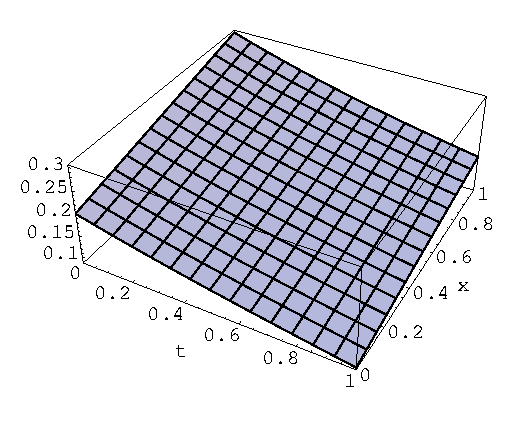
\includegraphics{senu_gr1.eps}}}%
\subfigure[]{
\resizebox*{5cm}{!}{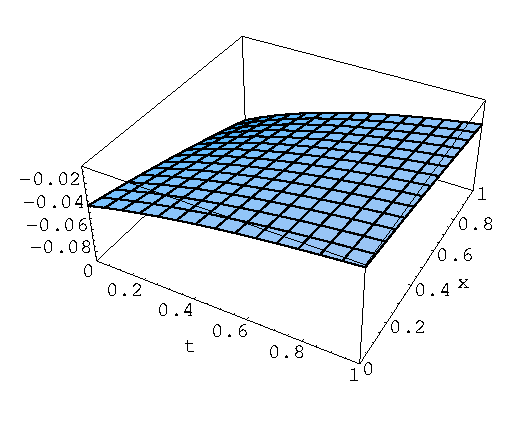
\includegraphics{senu_gr2.eps}}}%
\caption{\label{fig2} Example of a two-part figure with individual %
sub-captions showing that all lines of figure captions range left.}%
\label{sample-figure}
\end{minipage}
\end{center}
\end{figure}
\end{verbatim}

\begin{figure}
\begin{center}
\begin{minipage}{100mm}
\subfigure[]{
\resizebox*{5cm}{!}{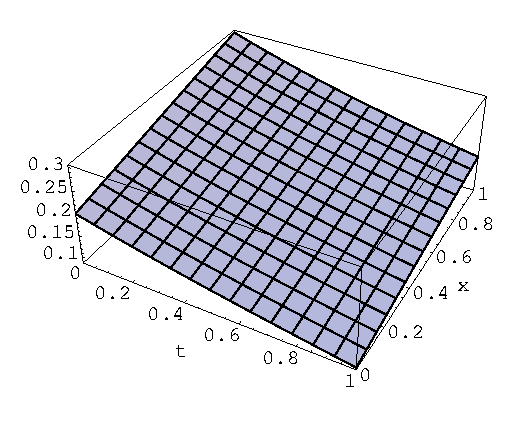
\includegraphics{senu_gr1.eps}}}%
\subfigure[]{
\resizebox*{5cm}{!}{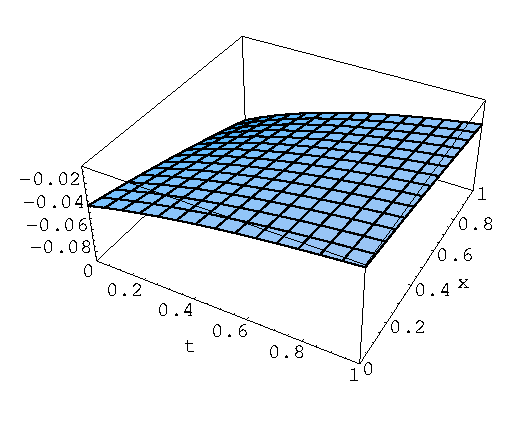
\includegraphics{senu_gr2.eps}}}%
\caption{Example of a two-part figure with individual %
sub-captions showing that all lines of figure captions range left.}%
\label{sample-figure}
\end{minipage}
\end{center}
\end{figure}

The control sequences \verb"\epsfig{}", \verb"\subfigure{}" and \verb"\includegraphics{}" require epsfig.sty,
subfigure.sty and graphicx.sty. These are called by the Class file {\tt tMAM2e.cls} and are included with the LaTeX
package for this journal for convenience.

To ensure that figures are correctly numbered automatically, the \verb"\label{}" command should be inserted just
after \verb"\caption{}"

\subsection{Tables}

The {\it tMAM} style will cope with most positioning of your tables
and you should not normally use the optional positional qualifiers
of the {\tt table} environment, which would override these
decisions. The table caption appears above the body of the table in
{\it tMAM} style, therefore the \verb"\tbl" command should appear
before the body of the table.

The {\tt tabular} environment can be used to produce tables with
single thick and thin horizontal rules, which are allowed, if
desired. Thick rules should be used at the head and foot only and
thin rules elsewhere.

Commands to redefine quantities such as \verb"\arraystretch"
should be omitted. For example, table~\ref{symbols} is produced
using the following commands. Note that \verb"\rm" will produce a
roman character in math mode. There are also \verb"\bf" and
\verb"\it", which produce bold face and text italic in math mode.
\begin{table}
  \tbl{Radio-band beaming model parameters
           for {FSRQs and BL Lacs.}}
{\begin{tabular}{@{}lcccccc}\toprule
   Class$^{\rm a}$
  & $\gamma _1$ & $\gamma _2$$^{\rm b}$
         & $\langle \gamma \rangle$
         & $G$ & $f$ & $\theta _{c}$ \\
\colrule
   BL Lacs &5 & 36 & 7 & $-4.0$
         & $1.0\times 10^{-2}$ & 10$^\circ$ \\
   FSRQs & 5 & 40 & 11 & $-2.3$
         & $0.5\times 10^{-2}$ & 14$^\circ$ \\
   \botrule
  \end{tabular}}
\tabnote{$^{\rm a}$This is not as accurate, owing to numerical
error.\\$^{\rm b}$An example table footnote to show the
text turning over when a long footnote is
inserted.}\label{symbols}
\end{table}

\begin{verbatim}
\begin{table}
  \tbl{Radio-band beaming model parameters
           for {FSRQs and BL Lacs.}}
{\begin{tabular}{@{}lcccccc}\toprule
   Class$^{\rm a}$
  & $\gamma _1$ & $\gamma _2$$^{\rm b}$
         & $\langle \gamma \rangle$
         & $G$ & $f$ & $\theta _{c}$ \\
\colrule
   BL Lacs &5 & 36 & 7 & $-4.0$
         & $1.0\times 10^{-2}$ & 10$^\circ$ \\
   FSRQs & 5 & 40 & 11 & $-2.3$
         & $0.5\times 10^{-2}$ & 14$^\circ$ \\
   \botrule
  \end{tabular}}
\tabnote{$^{\rm a}$This is not as accurate, owing to
          numerical error.}
\tabnote{$^{\rm b}$An example table footnote to show the
      text turning over when a long footnote is inserted.}%
      \label{symbols}
\end{table}
\end{verbatim}

To ensure that tables are correctly numbered automatically, the
\verb"\label{}" command should be inserted just before
\verb"\end{table}".

\subsection{Running headlines}\label{markboth}

In {\it tMAM} style, the authors' names and the title of the journal are used alternately throughout the article as a running headline at the top of each page. An abbreviated list of authors' names in italic format appears on even-numbered pages (versos)---e.g. `{\em J. Smith and P. Jones}', or `{\em J. Smith} et al.' for three or more authors, and the journal title in italic format is used on odd-numbered pages (rectos). To achieve this, the \verb"\markboth" command is used. The running headlines for this guide were produced using the following code:
\verb"\markboth{Taylor \& Francis and I.T. Consultant}{Journal of Mathematics"
\verb"and Music}". The \verb"\pagestyle" and \verb"\thispagestyle" commands should {\it not\/} be used.

\subsection{Maths environments}

The {\it tMAM} style provides for the following maths environments.

\begin{lemma}
More recent algorithms for solving the semidefinite programming
relaxation are particularly efficient, because they explore the structure
of the MAX-CUT.
\end{lemma}
\begin{theorem}
More recent algorithms for solving the semidefinite programming
relaxation are particularly efficient, because they explore the structure
of the MAX-CUT.
\end{theorem}
\begin{corollary}
More recent algorithms for solving the semidefinite programming
relaxation are particularly efficient, because they explore the
structure of the MAX-CUT.
\end{corollary}
\begin{proposition}
More recent algorithms for solving the semidefinite programming
relaxation are particularly efficient, because they explore the structure
of the MAX-CUT.
\end{proposition}
\begin{conjecture}
More recent algorithms for solving the semidefinite programming
relaxation are particularly efficient, because they explore the structure
of the MAX-CUT.
\end{conjecture}
\begin{example}
More recent algorithms for solving the semidefinite programming
relaxation are particularly efficient, because they explore the
structure of the MAX-CUT problem.
\end{example}
\begin{fact}
More recent algorithms for solving the semidefinite programming
relaxation are particularly efficient, because they explore the
structure of the MAX-CUT problem.
\end{fact}
\begin{remark}
More recent algorithms for solving the semidefinite programming
relaxation are particularly efficient, because they explore the
structure of the MAX-CUT problem.
\end{remark}
\begin{algorithm}
More recent algorithms for solving the semidefinite programming
relaxation are particularly efficient, because they explore the
structure of the MAX-CUT problem.
\end{algorithm}
\begin{proof}
More recent algorithms for solving the semidefinite programming
relaxation are particularly efficient, because they explore the structure
of the MAX-CUT.
\end{proof}
\noindent These were produced by:
\begin{verbatim}
\begin{lemma}
More recent algorithms for solving the semidefinite
programming relaxation are particularly efficient,
because they explore the structure of the MAX-CUT.
\end{lemma}

\begin{theorem}
...
...
\end{theorem}

\begin{corollary}
...
...
\end{corollary}

\begin{proposition}
...
...
\end{proposition}

\begin{conjecture}
...
...
\end{conjecture}

\begin{example}
...
...
\end{example}

\begin{remark}
...
...
\end{remark}

\begin{fact}
...
...
\end{fact}

\begin{algorithm}
...
...
\end{algorithm}

\begin{proof}
...
...
\end{proof}


\end{verbatim}


\subsection{Typesetting mathematics}\label{TMth}

\subsubsection{Displayed mathematics}

The {\it tMAM} style will set displayed mathematics centred on the
measure without equation numbers, provided that you use the \LaTeXe\
standard control sequences open (\verb"\[") and close (\verb"\]")
square brackets as delimiters. The equation
\[
  \sum_{i=1}^p \lambda_i = {\rm trace}({\textrm{\bf S}})\qquad
  i\in {\mathbb R}
\]
\normalfont was typeset in the {\it tMAM} style using the commands
%
\begin{verbatim}
\[
  \sum_{i=1}^p \lambda_i = {\rm trace}({\textrm{\bf S}})\qquad
  i\in {\mathbb R}
\].
\end{verbatim}

For those of your equations that you wish to be automatically
numbered sequentially throughout the text, use the {\tt{equation}}
environment, e.g.

\begin{equation}
  \sum_{i=1}^p \lambda_i = {\rm trace}({\textrm{\bf S}})\qquad
  i\in {\mathbb R}
\end{equation}

was typeset using the commands

\begin{verbatim}
\begin{equation}
  \sum_{i=1}^p \lambda_i = {\rm trace}({\textrm{\bf S}})quad
  i\in {\mathbb R}
\end{equation}
\end{verbatim}

Part numbers for sets of equations may be generated using the
{\tt{subequations}} environment, e.g.
\begin{subequations} \label{subeqnexample}
\begin{equation}
        \varepsilon \rho w_{tt}(s,t)
        =
        N[w_{s}(s,t),w_{st}(s,t)]_{s},
        \label{subeqnpart}
\end{equation}
\begin{equation}
        w_{tt}(1,t)+N[w_{s}(1,t),w_{st}(1,t)] = 0,
\end{equation}
\end{subequations}
which was generated using the control sequences

\begin{verbatim}
\begin{subequations} \label{subeqnexample}
\begin{equation}
        \varepsilon \rho w_{tt}(s,t)
        =
        N[w_{s}(s,t),w_{st}(s,t)]_{s},
        \label{subeqnpart}
\end{equation}
\begin{equation}
        w_{tt}(1,t)+N[w_{s}(1,t),w_{st}(1,t)] = 0,
\end{equation}
\end{subequations}
\end{verbatim}
This is made possible by the package {\tt{subeqn}}, which is called
by the Class file. If you put the \verb"\label{}" just after the
\verb"\begin{subequations}" line, references will be to the
collection of equations, `(\ref{subeqnexample})' in the example
above. Or, like the example code above, you can reference each
equation individually---e.g. `(\ref{subeqnpart})'.

\subsubsection{Bold math italic symbols}

To get bold math italic you can use \verb"\bm", which works for
all sizes, e.g.
%
\begin{verbatim}
\sffamily
\begin{equation}
   {\rm d}({\bm s_{t_{\bm u}}) = \langle{\bm\alpha({\sf{\textbf L}})}%
   [RM({\bm X}_y + {\bm s}_t) - RM({\bm x}_y)]^2 \rangle
\end{equation}
\normalfont
\end{verbatim}
%
produces\sffamily
\begin{equation}
   {\rm d}({\bm s_{t_{\bm u}}}) = \langle {\bm\alpha({\sf{\textbf L}})}[RM({\bm X}_y
   + {\bm s}_t) - RM({\bm x}_y)]^2 \rangle .
\end{equation}\normalfont
Note that subscript, superscript, subscript to subscript, etc.
sizes will take care of themselves and are italic, not bold,
unless coded individually. \verb"\bm" produces the same effect as
\verb"\boldmath". \verb"\sffamily"...\verb"\normalfont" allows
upright sans serif fonts to be created in math mode by using the
control sequence `\verb"\sf"'.



\subsubsection{Bold Greek}\label{boldgreek}

Bold lowercase as well as uppercase Greek characters can be
obtained by \verb"{\bm \gamma}", which gives ${\bm \gamma}$, and
\verb"{\bm \Gamma}", which gives ${\bm \Gamma}$.


\subsubsection{Upright lowercase Greek characters and the upright partial derivative sign}\label{upgreek}

Upright lowercase Greek characters can be obtained with the Class file by inserting the letter `u' in the control
code for the character, e.g. \verb"\umu" and \verb"\upi" produce $\umu$ (used, for example, in the symbol for the
unit microns---$\umu{\rm m}$) and $\upi$ (the ratio of the circumference to the diameter of a circle). Similarly,
the control code for the upright partial derivative $\upartial$ is \verb"\upartial".
\subsection{Acknowledgements}

An unnumbered section, e.g. \verb"\section*{Acknowledgement(s)}", should be used for thanks, grant details, etc.
and placed before any Notes or References sections.
\subsection{Notes}

An unnumbered section, e.g. \verb"\section*{Note(s)}", may be inserted after any Acknowledgements and before any References section.
\subsection{Appendices}

Appendices should be set after the references, beginning with the
command \verb"\appendices" followed by the command \verb"\section"
for each appendix title, e.g.
%
\begin{verbatim}
\appendices
\section{This is the title of the first appendix}
\section{This is the title of the second appendix}
\end{verbatim}

\noindent produces\medskip

\noindent Appendix A. This is the title of the first appendix

\noindent Appendix B. This is the title of the second appendix

\medskip
Subsections, equations, theorems, figures, tables, etc. within
appendices will then be automatically numbered as appropriate.
\subsection{References}\label{refs}

\subsubsection{References cited in the text} References cited in the text should be quoted by number (e.g.
[1], [2,4,10], [21--55], not [21]--[55]). References should be listed in {\tt{thebibliography}} environment in the order in which they first appear within the main text. Each bibliographical entry has a key, which is assigned by the author
and used to refer to that entry in the text. In this document, the key \verb"neu83" in the citation form
\verb"\cite{neu83}" produces `[1]', and the keys \verb"ed84" and \verb"aiex02" in the citation form
\verb"\cite{ed84,aiex00}" produce `[2, 3]'. The citation for a range of bibliographic entries (e.g.
`\cite{neu83,ed84,aiex00,aiex02,glov86,glov00,mtw73,hk96,fzf88,fwp88}') will automatically be produced by
\verb"\cite{neu83,ed84,aiex00,glov00,glov86,mtw73,hk96,fzf88,fwp88}". Optional notes may be included at the end of a citation by the use of square brackets, e.g. \verb"\cite[see][and references therein]{fzf88}" produces `\cite[see][and references therein]{fzf88}'.

\subsubsection{The list of references} The following listing shows some references prepared in the style of the
journal; note that references with more than ten authors begin with the first-named author's initials and
surname followed by `et al.'; references having the same author(s) are listed chronologically, beginning with the earliest.
%
%
\begin{thebibliography}{10}
\markboth{Taylor \& Francis and I.T. Consultant}{Journal of Mathematics and Music}
\bibitem[1]{neu83}%1
M. Neumann, {\em Parallel GRASP with path-relinking for job shop scheduling}, Mol. Phys. 50 (1983), pp. 841--843.

\bibitem[2]{ed84}%2
D.M.F. Edwards and I.R. McDonald, {\em Positive bases in numerical optimization}, Comput. Optim. Appl. 21 (1984),
pp. 169--175.

\bibitem[3]{aiex00}%3
R.M. Aiex, I.F. Pierce, G. Donizetti, C.M. {{v}on~Weber}, G. Bizet, C.P.E. Bach, R. Strauss, L. {{v}an~Beethoven}, W.A. Mozart, and P. Dukas, {\em Computing tools for modelling orchestral performance}, Tech.
Rep. DAMTP 2000/NA10, Department of Applied Mathematics and Theoretical Physics, University of Cambridge,
Cambridge, UK, 2000.

\bibitem[4]{aiex02}%4
R.M. Aiex et al.,  {\em Conjectured statistics for the {$q,t$}-Catalan numbers}, to appear in Advances in Math. (preprint 2002), Available at http://www.math.caltech.edu/$_{\huge{\tilde{}}}$rmaiex.

\bibitem[5]{glov86}%5
F. Glover,  {\em Hilbert modular forms and the Galois representations associated to Hilbert--Blumenthal abelian varieties}, Ph.D. diss., Harvard University, 1986.

\bibitem[6]{glov00}%6
F. Glover, {\it{Multi-start and strategic oscillation methods---principles to exploit adaptive memory}}, in {\it Computing Tools for Modeling, Optimization and Simulation: Interfaces in Computer Science and Operations Research}, M. Laguna and J.L. Gonz\'{a}les-Velarde, eds., 2nd ed., Kluwer Academic, Boston, MA, 2000, pp. 1--24.


\bibitem[7]{mtw73}%7
C.W. Misner (ed.), {\it{Proc. Symposia in Pure Math.}}, vol. 18, part 2, {\it{Nonlinear Operators and Nonlinear Equations of Evolution in Banach Spaces}}, Freeman, San \nobreak Francisco, CA, 1973, pp. 231--256.

\bibitem[8]{hk96}%8
H. Kern, {\em{The resurgent Japanese economy and a Japan--United States free trade agreement}}, in {\em{4th International Conference on the Restructuring of the Economic and Political System
in Japan and Europe}}, Milan, Italy, 21--25 May 1996, World Scientific, Singapore, 1997, pp. 147--156.

\bibitem[9]{fzf88}%9
F. French, {\em{English title of a chapter in the translation of a book in a foreign language}}, in {\itshape Title
of a Book in Another Language (Quoted in that Language)}, P. Smith (Transl.), Dover, New York, 1988 (original work
published 1923).

\bibitem[10]{fwp88}%10
F.W. Patel, {\itshape Title of a Book}, Monographs on Technical Aspects Vol. II, Dover, New York, 1988.

\bibitem[11]{GHGsoft}%11
T.G. Golda, P.D. Hough, and G. Gay, APPSPACK (Asynchronous parallel pattern search package); software available
at http://software.sandia.gov/appspack.
\markboth{Taylor \& Francis and I.T. Consultant}{Journal of Mathematics and Music}
\end{thebibliography}
\medskip
\noindent This list was produced by:
\vspace{6pt}
\begin{verbatim}
\begin{thebibliography}{10}

\bibitem[1]{neu83}%1
M. Neumann, {\em Parallel GRASP with path-relinking for job shop %
scheduling}, Mol. Phys. 50 (1983), pp. 841--843.

\bibitem[2]{ed84}%2
D.M.F. Edwards and I.R. McDonald, {\em Positive bases in numerical %
optimization}, Comput. Optim. Appl. 21 (1984),
pp. 169--175.

\bibitem[3]{aiex00}%3
R.M. Aiex, I.F. Pierce, G. Donizetti, C.M. {{v}on~Weber}, G. Bizet, %
C.P.E. Bach, R. Strauss, L. {{v}an~Beethoven}, W.A. Mozart, and P. %
Dukas, {\em Computing tools for modelling orchestral performance}, %
Tech. Rep. DAMTP 2000/NA10, Department of Applied Mathematics and %
Theoretical Physics, University of Cambridge, Cambridge, UK, 2000.

\bibitem[4]{aiex02}%4
R.M. Aiex et al.,  {\em Conjectured statistics for the %
{$q,t$}-Catalan numbers}, to appear in Advances in Math. (preprint %
2002), Available at http://www.math.caltech.edu/$_{\huge{\tilde{}}}$%
rmaiex.

\bibitem[5]{glov86}%5
F. Glover,  {\em Hilbert modular forms and the Galois representations %
associated to Hilbert--Blumenthal abelian varieties}, Ph.D. diss., %
Harvard University, 1986.

\bibitem[6]{glov00}%6
F. Glover, {\it{Multi-start and strategic oscillation methods---%
principles to exploit adaptive memory}}, in {\it Computing Tools %
for Modeling, Optimization and Simulation: Interfaces in Computer %
Science and Operations Research}, M. Laguna and J.L. Gonz\'{a}les-%
Velarde, eds., 2nd ed., Kluwer Academic, Boston, MA, 2000, pp. 1--24.


\bibitem[7]{mtw73}%7
C.W. Misner (ed.), {\it{Proc. Symposia in Pure Math.}}, vol. 18, %
part 2, {\it{Nonlinear Operators and Nonlinear Equations of Evolution %
in Banach Spaces}}, Freeman, San \nobreak Francisco, CA, 1973, pp. %
231--256.

\bibitem[8]{hk96}%8
H. Kern, {\em{The resurgent Japanese economy and a Japan--United %
States free trade agreement}}, in {\em{4th International Conference %
on the Restructuring of the Economic and Political System in Japan %
and Europe}}, Milan, Italy, 21--25 May 1996, World Scientific, %
Singapore, 1997, pp. 147--156.

\bibitem[9]{fzf88}%9
F. French, {\em{English title of a chapter in the translation of a %
book in a foreign language}}, in {\itshape Title of a Book in Another %
Language (Quoted in that Language)}, P. Smith (Transl.), Dover, New %
York, 1988 (original work
published 1923).

\bibitem[10]{fwp88}%10
F.W. Patel, {\itshape Title of a Book}, Monographs on Technical %
Aspects Vol. II, Dover, New York, 1988.

\bibitem[11]{GHGsoft}%11
T.G. Golda, P.D. Hough, and G. Gay, APPSPACK (Asynchronous parallel %
pattern search package); software available at http://software.sandia.
gov/appspack.

\end{thebibliography}
\end{verbatim}

\medskip
\noindent Each entry takes the form:
\medskip
\begin{verbatim}
\bibitem{key} Bibliography entry
\end{verbatim}
%
where {\tt key} is the tag that is to be used as an argument for the \verb"\cite{}" command. {\tt Bibliography
entry} should be the material that is to appear in the bibliography, suitably formatted.\bigskip

Instead of including `thebibliography' environment in the main source file of their article, authors may include
the lines \vspace{12pt}

\noindent\verb"\bibliographystyle{tMAM}"
\newline\verb"\bibliography{tMAMguide}"
\vspace{12pt}

\noindent where the references list should appear, where tMAM.bst is the BiBTeX style file for this journal and
tMAMguide.bib is the database of bibliographic details for the references section (both included with the tMAM
LaTeX style guide package). tMAMguide.bib can be used as a template for creating your database, which can be
used with any of your future papers. The \LaTeXe\ source file of a particular paper will extract from the .bib
file only those references that are cited in that paper and listed in the references section of it.
Thus\vspace{12pt}

\noindent\verb"\bibliographystyle{tMAM}"
\newline\verb"\bibliography{tMAMguide}"
\vspace{12pt}

\noindent produces:\\\vspace{-50pt}
\bibliographystyle{tMAM}
\bibliography{tMAMguide}
 \vspace{36pt}

\noindent Note that only ten of the eleven bibitems in the .bib file have appeared in the above references list
because these are the only ten cited in the text of this guide.

\markboth{Taylor \& Francis and I.T. Consultant}{Journal of Mathematics and Music}
\subsection{{\bi tMAM} macros}

Table~\ref{macros} gives a list of macros for use with {\it tMAM}.
The list displays each macro's code and a description/demonstration
of its function.

\begin{table} \tbl{{\it tMAM} macros.}{\begin{tabular}{@{}ll}\toprule
$\backslash$markboth\{short author(s) list\}\{short journal title\}& short author(s) list and short journal title\\
& in running heads (verso/recto,
resp.)\\\cr
$\backslash$thanks\{title-page footnote to article title & e.g. `Corresponding author. E-mail:\\
or author\} & A.N. Author@uiowa.edu'\\\cr

$\backslash$begin\{abstract\}...$\backslash$end\{abstract\} & for
abstract on titlepage\\\\ $\backslash$bm\{math and symbols\} &
bold italic $\bm{math\;and\;symbols}$\\\cr $\backslash$bi\{text\}
& bold italic \bi{text}\\\cr $\backslash$sf\{text or upright
symbols in math mode\} & sans serif \sf{text} or
$\sf{upright\;symbols\;in\;math\;mode}$
\\\botrule
\end{tabular}}
\label{macros}
\end{table}

\section{Example of a section heading with\\*
   {\fontencoding{T1}\scshape\lowercase{small caps}},
   \lowercase{lowercase}, {\bi italic},
   and bold\\* Greek such as
   ${\bm\kappa}$}\label{headings}

%
The following code shows how to achieve this section head:
%
\begin{verbatim}
\section{Example of section heading with\\*
   {\fontencoding{T1}\scshape\lowercase{small caps}},
   \lowercase{lowercase}, {\bi italic},
   and bold\\* Greek such as
   ${\bm\kappa}$}\label{headings}
\end{verbatim}
%
%
%%%%%%%%%%%%%%%%%%%%%%%%%%%%%%%%%%%%

\section{{\textit{tMAM}} journal style}

The notes given here relate to common style errors found in  {{\it
tMAM}} manuscripts, but are {\itshape not\/} intended to be
exhaustive.

\subsection{Punctuation}

When  deciding  where to add commas, it may be  helpful  to  read
through  the sentence and note where the natural `pauses'  occur.
The  needs  of readers for whom English is not a  first  language
should  be  borne in mind when punctuating  long  sentences.  For
example, consider the following sentence as it appeared in {\it
tMAM}: `When we do not limit ourselves by constraints arising from
the choice of an initial fluctuation spectrum, structures in an open
universe, including the peculiar velocity structure,  can be
reproduced  in a flat Lema\^{\i}tre universe for a large  part of
their evolution.' Now consider the same sentence without commas:
`When  we do not limit ourselves by constraints arising from  the
choice  of an initial fluctuation spectrum structures in an  open
universe including the peculiar velocity structure can be reproduced
in  a  flat Lema\^{\i}tre universe for a large  part of  their
evolution.'

\subsection{Spelling}

Please use either British spelling (e.g.\ centre not center, labelled not  labeled, with -ise endings for devise,  surprise, comprise, revise and exercise, the -yse ending for analyse, and -ize endings for recognize, criticize, minimize, emphasize and organize) or US spelling. If the manuscript received uses a mixture of UK and American spelling, it will be edited into consistently UK spelling.

\subsection{Hyphens, n-rules, m-rules and minus signs}

\begin{enumerate}
\item[(i)] Hyphens (one dash in \TeX/\LaTeXe). {\it tMAM} uses hyphens
for compound adjectives (e.g.\ low-density gas, least-squares fit,
two-component  model) but not for complex  units  or ranges, which
could become cumbersome (e.g.\ 15~km~s$^{-1}$  feature,
100--200~$\umu$m observations).

\item[(ii)] n-rules (two dashes in \TeX/\LaTeXe). These are used  (a) to denote a range (e.g.\
1.6--2.2~$\umu$m); and (b) to denote the joining of two words of
equal standing (e.g.\ Kolmogorov--Smirnov  test, Herbig--Haro
object).

\item[(iii)] The  m-rule (three dashes in \TeX/\LaTeXe) is  used  in
{\it tMAM} as an alternative to parentheses (e.g.\  `the
results---assuming no temperature gradient---are indicative of
\ldots').
\item[(iv)] The minus sign (one dash in \TeX/\LaTeXe) is produced
automatically in math mode by use of a single dash, e.g.
\begin{equation}
y_{i} \in \{-1, 1 \} \quad \forall i \in V
\end{equation}
\noindent where $|-V|=A^2+B^2$\medskip

\noindent is produced by

\begin{verbatim}
\begin{equation}
y_{i} \in \{-1, 1 \} \quad \forall i \in V
\end{equation}
\noindent where $|-V|=A^2+B^2$
\end{verbatim}

\end{enumerate}


\subsection{References}

It is important to use the correct reference style, details  of which can be found in Section~\ref{refs} above.

\subsection{Maths fonts}
Scalar  variables should be mediumface italic (e.g. $s$ for
speed); vectors should be bold italic (e.g. $\bm v$ for velocity);
matrices should be bold roman (upright) (e.g. $\bf A$), and
tensors should be bold upright sans serif (e.g. {\sffamily{\textbf
L}}). Differential d, partial differential $\upartial$, complex i,
exponential e, superscript T for `transpose', sin, cos, tan, log,
etc., should all be roman. Openface, or `blackboard', fonts can be
used, for example, for the integers $\mathbb Z$ and the reals
$\mathbb R$. Sub/superscripts that are physical variables should
be italic, while those  that are labels should be roman (e.g.\
$C_p$, $T_{\rm eff}$). Displayed equations should have end-of-line
punctuation appropriate to the running text sentence of which they
form a part.


\section{Troubleshooting}

Authors may from time to time encounter problems with the  preparation
of their papers in \LaTeXe. The appropriate  action  to
take will depend on the nature of the problem -- the following is
intended to act as a guide.
%
\begin{enumerate}
\item[(i)] If the problem is with \LaTeXe\ itself, rather than with the
actual macros, please refer to the appropriate handbooks for
initial advice.\footnote{\TeX: Knuth, D., 1986, {\it The \TeX\
book} (New York: Addison--Wesley); \LaTeXe: Lamport, L., 1985,
{\it \LaTeXe\ \nobreak User's Guide and Reference Manual} (New
York: Addison--Wesley).} If the solution cannot be found, and you
suspect that the problem lies with the macros, then please contact
Taylor \& Francis ({\tt latex.helpdesk@tandf.co.uk}).

\item[(ii)] Problems with page make-up (e.g.\ large spaces between paragraphs, or under headings or
figures; uneven columns; figures/tables appearing out of order):
please do {\itshape not\/} attempt to remedy these yourself using
`hard' page make-up commands -- the typesetter will correct such
problems. (You may, if you wish, draw attention to particular
problems when submitting the final version of your paper.)

\item[(iii)] If a required font is not available at your site, allow \TeX\
to substitute the font and specify which font your require in the
covering letter accompanying your file(s).

\end{enumerate}


\subsection{Fixes for coding problems}

This guide has been designed to minimize the need for user-defined macros to  create special symbols. Authors
are urged, wherever possible, to use the following coding rather than to create their own. This will minimize
the danger of author-defined macros being accidentally  `over-ridden' when the paper is typeset in Times (see
Section~\ref{TMth}, `Typesetting mathematics' above). In cases where it is essential to create your own macros,
these should be displayed in the preamble of the source file before \verb"\begin{document}".

%
\begin{enumerate}
\item[(i)] Fonts in section headings and paper titles. The following are  examples
of styles that sometimes prove difficult to code.


\subsection*{P\lowercase{aper titles:}}

\hsize380pt\bf{\noindent Generalized Flory theory at ${\bm\delta >
{\bf
   50}^\circ}$}\\

    \noindent\normalfont is produced by
\begin{verbatim}
\title{Generalized Flory theory at
        ${\bm\delta > {\bfseries 50}^\circ}$}
\end{verbatim}
\bigskip

{\bf{\noindent Ion--ion correlations in H\,{\sc ii} regions}}\\

\noindent\normalfont is produced by
%
\begin{verbatim}
\title{Ion--ion correlations in H\,{\sc ii} regions}
\end{verbatim}


\stepcounter{enumi}

\item[(ii)] n-rules, m-rules, hyphens and minus signs (see Section~6.3 for
correct usage). To create the correct symbols in the sentence
%
\begin{quote}
The high-resolution observations were made along a line at an
angle of $-15^\circ$ (East from North) from the axis of the
jet---which runs North--South
\end{quote}
you would use the following code:
%
\begin{verbatim}
The high-resolution observations were made along a line at an
angle of $-15^\circ$ (East from North) from the axis of the
jet---which runs North--South
\end{verbatim}

\item[(iii)] Fonts in superscripts and subscripts. Subscripts and superscripts will automatically come  out in the correct font
and size in a math environment (e.g. enclosed by `\verb"$"'
delimiters in running text or within \verb"\[...\]" or the
`equation' environment for displayed equations). You can create
the output ${\bm k_x}$ by typing \verb"${\bm k_x}$". If the
subscripts or superscripts need to be other than italic, they
should be coded individually---see (vi) below.

\item[(iv)] Calligraphic letters (uppercase only).
%
%
Normal calligraphic can be produced with \verb"\cal" as usual (in
math mode).

\item[(v)] Automatic scaling of brackets. The codes \verb"\left" and
\verb"\right" should  be used to scale brackets automatically to
fit the equation being set. For example, to get
\[
   v = x \left( \frac{N+2}{N} \right)
\]
use the code
%
\begin{verbatim}
\[
   v = x \left( \frac{N+2}{N} \right)
\]
\end{verbatim}

\item[(vi)] Roman font in equations. It is often necessary to make some
symbols roman in an equation (e.g.\ units, non-variable
subscripts). For example, to get the following output:
\[
   \sigma \simeq (r/13~h^{-1}~{\rm Mpc})^{-0.9},
   \qquad \omega = \frac{N-N_{\rm s}}{N_{\rm R}}
\]
\noindent you should use:
%
\begin{verbatim}
\[
   \sigma \simeq (r/13~h^{-1}
   ~{\rm Mpc})^{-0.9}, \qquad \omega
   =\frac{N-N_{{\rm s}}}{N_{{\rm R}}}
\]
\end{verbatim}
\end{enumerate}

\section{Obtaining the tMAM2e Class file}\label{FTP}

\subsection{Via the Taylor \& Francis website}

\noindent This Guide for Authors and the {\tt tMAM2e.cls} Class file may be obtained via the Instructions for Authors on the Taylor \& Francis homepage for the journal ({\tt{http://www.tandf.co.uk/journals/titles/17459737.asp}}).

Please note that the Class file calls up the following open-source LaTeX packages, which will, for convenience, unpack with the downloaded Guide for Authors and Class file: amsbsy.sty, amsfonts.sty, amsmath.sty, amssymb.sty, enumerate.sty, epsfig.sty, graphicx.sty, mathbbol.sty, natbib.sty, rotating.sty, subfigure.sty.

\subsection{Via e-mail}

This Guide for Authors, the Class file and the associated open-source LaTeX packages are also available by e-mail. Requests should be addressed to {\tt latex.helpdesk@tandf.co.uk} clearly stating for which journal you require the Guide for Authors and/or Class file.

%%%%%%%%%%%%%%%%%%%%%%%%%%%%%%%%%%%%

\label{lastpage}

\end{document}
